\documentclass[border=8pt]{standalone}
\usepackage{pgfplots}
\usepgfplotslibrary{fillbetween}
\pgfplotsset{compat=1.18}
\begin{document}
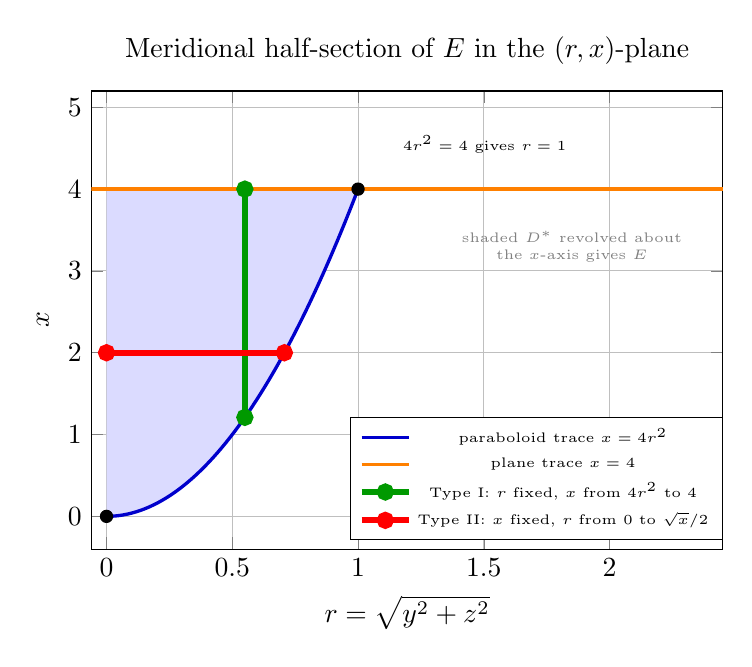
\begin{tikzpicture}
\begin{axis}[
    width=9.6cm, height=7.4cm,
    xlabel={$r=\sqrt{y^{2}+z^{2}}$}, ylabel={$x$},
    xmin=-0.06, xmax=2.45, ymin=-0.4, ymax=5.2,
    xtick={0,0.5,...,2.5}, ytick={0,1,...,5},
    grid=major,
    title={Meridional half-section of $E$ in the $(r,x)$-plane},
    legend style={font=\tiny, at={(1.0,0.02)}, anchor=south east},
]
% helper paths (not drawn, not listed in legend)
\addplot[name path=par, draw=none, forget plot, domain=0:1, samples=60] {4*x^2};
\addplot[name path=cup, draw=none, forget plot, domain=0:1, samples=2] {4};
% shade the region 4r^2 <= x <= 4
\addplot[blue!14, forget plot] fill between[of=par and cup];

\addplot[blue!80!black, very thick, domain=0:1, samples=60] {4*x^2};
\addlegendentry{paraboloid trace $x=4r^{2}$}
\addplot[orange, very thick, domain=-0.06:2.45, samples=2] {4};
\addlegendentry{plane trace $x=4$}
\addplot[black, only marks, mark=*, mark size=2.2pt, forget plot] coordinates {(1,4) (0,0)};
\addplot[green!60!black, line width=2.2pt, mark=*] coordinates {(0.55,1.21) (0.55,4)};
\addlegendentry{Type I: $r$ fixed, $x$ from $4r^{2}$ to $4$}
\addplot[red, line width=2.2pt, mark=*] coordinates {(0,2) (0.7071,2)};
\addlegendentry{Type II: $x$ fixed, $r$ from $0$ to $\sqrt{x}/2$}
\node[font=\tiny, anchor=west] at (axis cs:1.14,4.55) {$4r^{2}=4$ gives $r=1$};
\node[font=\tiny, align=center, gray] at (axis cs:1.85,3.3)
     {shaded $D^{*}$ revolved about\\ the $x$-axis gives $E$};
\end{axis}
\end{tikzpicture}
\end{document}
